\section{MF Ranking Model}
\label{chap:tree-ranking:mf-model}

In general, an entity contains some structure which provides relevant information about its content. For example, an entity that describes a book would be divided into chapters, each chapter into sections, each section into a set of paragraphs. In order to retain this structure for later use in the ranking, we generalize field-based approaches with the ``MF'' ranking model for Directed Acyclic Graphs (DAG) by integrating the complete graph structure into its model.

First, we present the revised entity model and introduce the formal model of MF. Next we present two extensions to the MF model. Finally, we describe weights developed for the MF model.

\subsection{Model}

In traditional field-based ranking models, an entity is modelled as a set of fields, each being a \emph{bag of words}. However in doing so, the rich structure of the entity is lost. For example, in Figure~\ref{fig:concept-tree} where the graph of an entity rooted in $N_0$ is depicted, we can create three fields, one for each attribute $a$, $b$, and $c$; the label of nodes are then distributed as follows:
\begin{itemize}
	\item $N_1$ is assigned to field $a$;
	\item $N_2$, $N_4$, and $N_5$ are assigned to field $b$; and
	\item $N_3$ and $N_4$ are assigned to the field $c$.
\end{itemize}
However, a shortcoming is that the relationship between nodes is discarded within a field. Indeed, in traditional field-based ranking models, most of the entity's structure is discarded.\\

Rather that representing the entity as a set of fields, the MF ranking model follows the structure of the graph. Each node of the graph --- not a set of nodes --- is represented as a bag of words. This allows to capture the graph's structure into the ranking model.

\paragraph{Eliteness.}

In \cite{harter:1974:thesis}, Harter introduced the notion of \emph{eliteness} in order to model content-bearing terms: a document is said to be \emph{elite} in term $t$ if it is somehow ``about'' the topic associated with $t$. In \cite{robertson:1981:PMI}, Robertson et al. introduce the relationship between the eliteness of a term in a document and its frequency: an elite term is most likely to be reused in the document, hence the term frequency is used as evidence of the term eliteness in the document.

In \cite{zaragoza:2004:microsoft}, Zaragoza et al. extend the notion of eliteness to documents with multiple fields. In \cite{robertson:2004:cikm}, the authors argue that the normalized frequencies of a term in each field should be combined before applying the term weighting model.

Similarly in our MF model, the term eliteness in an entity is shared between its attributes. The values related to a same attribute are associated to a same topic, described by the edge label. Therefore, a term eliteness in an attribute is shared between its values. For nested entities that are more than a hop away from the root, the same interpretation applies.\\

In the following paragraphs, we describe how the term eliteness is garnered from every node of the entity description.

\paragraph{Expanded entity graph.}

Our model revolves around two core operations: on the one hand, the importance of an entity with regards to a query is computed on the leaves; on the other hand, internal nodes are used for aggregating the scores. In order to take into account
\begin{inparaenum}[(a)]
	\item the label of internal nodes; and
	\item the label of edges,
\end{inparaenum}
we expand the graph so that each label becomes a leaf. To do so, we transform the entity graph into a graph where each label --- edge and node --- is a node, as depicted in Figure~\ref{fig:expanded-graph1}. Then, each node of that transformed graph becomes a leaf of the tree, as depicted in Figure~\ref{fig:expanded-graph2}; this is the expanded entity graph of the entity in Figure~\ref{fig:concept-tree}.

\begin{figure}
	\centering
	\begin{subfigure}{.3\textwidth}
		\centering
		\resizebox{\textwidth}{!}{
			\begin{tikzpicture}[->,>=stealth',every node/.style={draw,circle},node distance=2cm]
\node (0) {$v_0$};
\node[below left of = 0] (1) {$v_1$};
\node[below of = 0] (2) {$v_2$};
\node[below right of = 0] (3) {$v_3$};
\node[below of = 3] (4) {$v_4$};
\node[below of = 2] (5) {$v_5$};

\path[every node/.style={font=\footnotesize,fill=white}]
(0) edge node {a} (1)
 edge node {b} (2)
 edge node {c} (3)
(3) edge node {d} (4)
(2) edge node {d} (5)
 edge node {d} (4)
;
\end{tikzpicture}
		}
		\caption{An entity description represented as a DAG. The root of the entity is the node $N_0$}
		\label{fig:concept-tree}
	\end{subfigure}
	\quad
	\begin{subfigure}{.3\textwidth}
		\centering
		\resizebox{\textwidth}{!}{
			\usetikzlibrary{positioning}

\begin{tikzpicture}[every node/.style={draw,circle},node distance=.8cm]

\node (0) {$v_0$};
\node[dashed,below left = of 0 ] (a) {a};
\node[dashed,below = of 0 ] (b) {b};
\node[dashed,below right = of 0 ] (c) {c};

\node[below = of a ] (1) {$v_1$};
\node[below = of b ] (2) {$v_2$};
\node[below = of c ] (3) {$v_3$};

\node[dashed,below = of 2 ] (d2) {d};
\node[dashed,below = of 3 ] (d3) {d};

\node[below = of d3 ] (4) {$v_4$};
\node[below = of d2 ] (5) {$v_5$};

\path[->,every node/.style={font=\footnotesize,fill=white}]
(0) edge (a)
	edge (b)
	edge (c)
(a) edge (1)
(b) edge (2)
(c) edge (3)
(2) edge (d2)
(3) edge (d3)
(d2) edge (4) edge (5)
(d3) edge (4)
;

\end{tikzpicture}
		}
		\caption{The graph of the entity in Figure~\ref{fig:concept-tree} where each label --- of a node and an edge alike --- becomes a node}
		\label{fig:expanded-graph1}
	\end{subfigure}
	\qquad
	\begin{subfigure}{.7\textwidth}
		\centering
		\resizebox{\textwidth}{!}{
			\usetikzlibrary{positioning}

\begin{tikzpicture}[->,circ/.style={draw,circle},node distance=.8cm]

\node (agg0) {$*$};

\path (agg0) ++(-150:3) node[circ] (0) {$N_0$};

\path (agg0) ++(-120:3) node (agg1) {$*$} ++(-110:2) node[dashed,circ] (a) {a};
\path (agg1) ++(-70:2) node[circ] (1) {$N_1$};

\path (agg0) ++(-60:3) node (agg2) {$*$} ++(-130:1.5) node[dashed,circ] (b) {b};
\path (agg2) ++(-50:1.5) node[circ] (2) {$N_2$};
\path (agg2) ++(-90:2) node (agg4) {$*$};

\path (agg4) ++(-130:2) node[dashed,circ] (d2) {d};
\path (agg4) ++(-90:2) node[circ] (5) {$N_5$};
\path (agg4) ++(-40:2.3) node[circ] (4) {$N_4$};

\node[right = 3cm of agg2] (agg3) {$*$};
\path (agg3) ++(-130:1.5) node[dashed,circ] (c) {c};
\path (agg3) ++(-50:1.5) node[circ] (3) {$N_3$};
\path (agg3) ++(-90:2) node (agg5) {$*$} ++(-90:1.5) node[dashed,circ] (d3) {d};

\path[every node/.style={font=\footnotesize,fill=white}]
(agg0) edge (0)
	edge (agg1)
	edge (agg2)
	edge (agg3)
(agg1) edge (a)
	edge (1)
(agg2) edge (b)
	edge (2)
	edge (agg4)
(agg3) edge (c)
	edge (3)
	edge (agg5)
(agg4) edge (d2)
	edge (4)
	edge (5)
(agg5) edge (d3)
	edge (4)
;

\end{tikzpicture}
		}
		\caption{The expanded graph of the entity in Figure~\ref{fig:concept-tree} where each node of the graph in Figure~\ref{fig:expanded-graph1} becomes a leaf. Nodes labelled with $*$ depict aggregations.}
		\label{fig:expanded-graph2}
	\end{subfigure}
	\caption{Depiction of the MF model}
\end{figure}

\paragraph{Algorithm.}

The score of an entity with regards to a query is computed with a bottom-up approach. The leaves of the entity's DAG contain information about the entity; a function that leverage the content and which returns a numerical value is then applied on that level. The internal nodes of the DAG aggregates the values computed on its outgoing nodes using a second function; the aggregation continues until the root of the entity is reached.

For instance, we compute the contribution of the leaves ``$d$'', ``$N_5$'', and ``$N_4$'', which are aggregated on the parent node. The aggregated value is then combined with its sibling nodes, i.e., ``$b$'' and ``$N_2$''. These operations are repeated until the root of the tree is reached.

\paragraph{MF Model Normalisations.}
\label{chap:tree-ranking:mf-model:norm}

Ranking models use statistics garnered from the entity to estimate its relevance with regards to a query. For instance, the frequency of a term can be used as an indicator for its importance in describing the entity. However, the entity is part of a dataset and the significance of the frequency as a measure varies between entities. This variability may be due to several factors, e.g., the writing style: two entities can provide the same amount of information about a certain topic, but one uses twice as much terms as the other.

In order to account for this variability in the dataset, there is a need for \emph{normalising}~\cite{manning:2008:iir} the statistics garnered from the entity. For instance, in BM25F~\cite{zaragoza:2004:microsoft} the frequency of a term within a field is normalised based on
\begin{inparaenum}[(a)]
	\item the length of the field; and
	\item the average length of the field within the dataset.
\end{inparaenum}
Thanks to the normalisation, it is possible to compare the relevance with regards to a query of entities within a dataset.\\

With traditional field-based ranking models, there is one level of normalisation that is performed on the content level, as discussed in the previous paragraph.
We can provide an additional normalisation, making two possible levels of normalisations with the MF ranking model:
\begin{enumerate}
	\item a normalisation on the \emph{content} level to account for the variability of a node's length within a dataset; and
	\label{norm:content}
	\item a normalisation of the outgoing \emph{degree} of a node.
	\label{norm:degree}
\end{enumerate}
The first normalisation is applied on the \emph{leaf} nodes of the DAG. The second normalisation is applied on the \emph{internal} nodes during the aggregation step. This additional level of normalisation allows a finer tuning of the ranking function.

%\begin{figure}[t]
%    \centering
%%    \begin{subfigure}{0.3\textwidth}
%%    	\centering
%%      	\begin{tikzpicture}[->,>=stealth',every node/.style={draw,circle},node distance=2cm]
\node (0) {$v_0$};
\node[below left of = 0] (1) {$v_1$};
\node[below of = 0] (2) {$v_2$};
\node[below right of = 0] (3) {$v_3$};
\node[below of = 3] (4) {$v_4$};
\node[below of = 2] (5) {$v_5$};

\path[every node/.style={font=\footnotesize,fill=white}]
(0) edge node {a} (1)
 edge node {b} (2)
 edge node {c} (3)
(3) edge node {d} (4)
(2) edge node {d} (5)
 edge node {d} (4)
;
\end{tikzpicture}
%%    	\caption{An entity represented as a tree with varying degree.}
%%		\label{fig:concept-tree}
%%    \end{subfigure}
%%  	\quad
%  	\begin{subfigure}{0.3\textwidth}
%  		\centering
%  		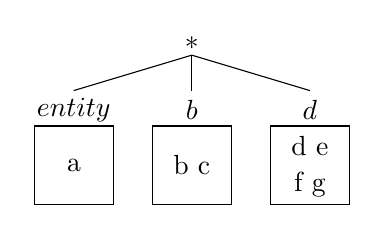
\begin{tikzpicture}
% field entity
\node at (-1,1.2) {$entity$};
\node at (-1,.5) {a};
\draw (-1.5,0) rectangle (-.5,1);
% field b
\node at (.5,1.2) {$b$};
\node at (.5,.5) {b c};
\draw (0,0) rectangle (1,1);
% field d
\node at (2,1.2) {$d$};
\node at (2,.75) {d e};
\node at (2,.25) {f g};
\draw (1.5,0) rectangle (2.5,1);
% Aggregate contributions of each field
\node at (.5,2) {*};
\draw (.5,1.9) -- (-1,1.45);
\draw (.5,1.9) -- (.5,1.45);
\draw (.5,1.9) -- (2,1.45);
\end{tikzpicture}
%  		\caption{Field-based ranking model for the entity. The $*$ symbolises the aggregation of the contribution of each child node, here a field.}
%		\label{fig:field-model}
%  	\end{subfigure}
%  	\quad
%  	\begin{subfigure}{0.3\textwidth}
%  		\centering
%  		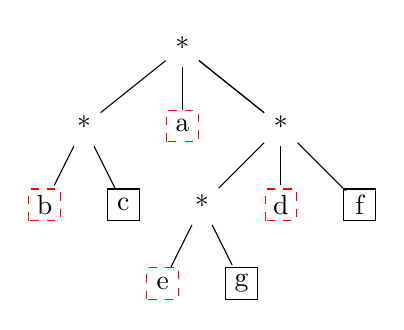
\begin{tikzpicture}
\node (a) at (-.25,0) {*};
\node (labela) at (-.25,-1) {a};
\node (b) at (-1.5,-1) {*};
\node (labelb) at (-2,-2) {b};
\node (c) at (-1,-2) {c};
\node (d) at (1,-1) {*};
\node (labeld) at (1,-2) {d};
\node (e) at (0,-2) {*};
\node (labele) at (-.5,-3) {e};
\node (f) at (2,-2) {f};
\node (g) at (.5,-3) {g};

\draw (a) -- (labela);
\draw (a) -- (b) -- (c);
\draw (b) -- (labelb);
\draw (d) -- (labeld);
\draw (e) -- (labele);
\draw (a) -- (d) -- (e) -- (g);
\draw (a) -- (d) -- (f);

\draw [red, dashed] (-2.2,-2.2) rectangle (-1.8,-1.8);
\draw (-1.2,-2.2) rectangle (-.8,-1.8);
\draw [red, dashed] (-.45,-1.2) rectangle (-.05,-.8);
\draw [red, dashed] (.8,-2.2) rectangle (1.2,-1.8);
\draw (1.8,-2.2) rectangle (2.2,-1.8);
\draw [red, dashed] (-.7,-3.2) rectangle (-.3,-2.8);
\draw (.3,-3.2) rectangle (.7,-2.8);
\end{tikzpicture}
%  		\caption{The MF ranking model for the entity. A square symbolizes where the contribution of a query term is performed. Red dashed squares represents internal nodes in the entity tree that were transformed into a leaf.}
%		\label{fig:mf-model}
%  	\end{subfigure}
%  	\quad
%  	\begin{subfigure}{\textwidth}
%  		\centering
%	  	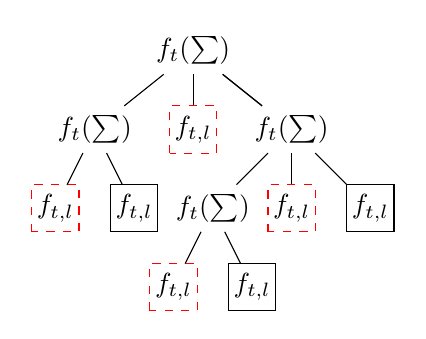
\begin{tikzpicture}
\node (a) at (-.25,0) {$f_{t}(\sum)$};
\node (labela) at (-.25,-1) {$f_{t,l}$};
\node (b) at (-1.5,-1) {$f_{t}(\sum)$};
\node (labelb) at (-2,-2) {$f_{t,l}$};
\node (c) at (-1,-2) {$f_{t,l}$};
\node (d) at (1,-1) {$f_{t}(\sum)$};
\node (labeld) at (1,-2) {$f_{t,l}$};
\node (e) at (0,-2) {$f_{t}(\sum)$};
\node (labele) at (-.5,-3) {$f_{t,l}$};
\node (f) at (2,-2) {$f_{t,l}$};
\node (g) at (.5,-3) {$f_{t,l}$};

\draw (a) -- (labela);
\draw (a) -- (b) -- (c);
\draw (b) -- (labelb);
\draw (d) -- (labeld);
\draw (e) -- (labele);
\draw (a) -- (d) -- (e) -- (g);
\draw (a) -- (d) -- (f);

\draw [red, dashed] (-2.3,-2.3) rectangle (-1.7,-1.7);
\draw (-1.3,-2.3) rectangle (-.7,-1.7);
\draw [red, dashed] (-.55,-1.3) rectangle (.05,-.7);
\draw [red, dashed] (.7,-2.3) rectangle (1.3,-1.7);
\draw (1.7,-2.3) rectangle (2.3,-1.7);
\draw [red, dashed] (-.8,-3.3) rectangle (-.2,-2.7);
\draw (.2,-3.3) rectangle (.8,-2.7);
\end{tikzpicture}
%  		\caption{Normalized term frequency computation in the MF ranking for the entity.}
%  		\label{fig:mf-ranking}
%  	\end{subfigure}
%	\caption{Abstract models for ranking a tree.}
%	\label{fig:tree}
%\end{figure}

\subsection{MF Ranking Functions}
\label{sec:mf-function}

In this section, we describe \emph{BM25MF} and \emph{PL2MF}, the MF extensions of BM25F~\cite{zaragoza:2004:microsoft} and PL2F~\cite{macdonald:2005:clef}, respectively.
We present first the features needed for the MF ranking model and then define both extensions.

\paragraph{Ranking features.}

The MF model introduces two levels of normalisations. In order to implement them, the following features are needed:

\subparagraph{Features for Normalisation~\ref{norm:content}.}

\begin{labeling}{\textbf{average leaf length:}}
  \item[\textbf{leaf length:}] refers to the number of terms in the label of a leaf;
  \item[\textbf{average leaf length:}] is the mean of the \emph{leaf length} of sibling nodes for a particular attribute;
\end{labeling}

\subparagraph{Features for Normalisation~\ref{norm:degree}.}

\begin{labeling}{\textbf{average attribute cardinality:}}
  \item[\textbf{attribute cardinality:}] is equal to the number of values an attribute possesses;
  \item[\textbf{average attribute cardinality:}] is equal to the mean of the \emph{attribute cardinality} across the entities where that attribute appears.
\end{labeling}

\subsubsection{BM25MF}
\label{sec:bm25mf-function}

BM25F is extended by adapting the Equation (\ref{eq:bm25f_1}). The resulting normalised term frequency is then passed to the saturation function in the Equation (\ref{eq:bm25f_2}).
The computation of the entity score with BM25MF consists of applying two functions, $f_{t,L}$ and $f_{t,I}$, applied on a leaf and on an internal node, respectively.\\

The BM25MF ranking function is defined following the two levels of normalisations.
The $f_{t,L}$ function implements the Normalisation~\ref{norm:content} on the content and is defined as follows:
\begin{equation}
\label{bm25mf_v}
f_{t,L} = \frac{\alpha_v\times F_t}{1+b_v\times\left(\frac{l}{l_a}-1\right)}
\end{equation}
in which the following notations are used:
\begin{itemize}
	\item $F_t$ is the frequency of the term $t$ within the leaf;
	\item $l$ is the \emph{leaf length} of the leaf; and
	\item $l_a$ is the \emph{average leaf length}.
	\item $\alpha_v$ is a weight specific to a leaf; and
	\item $b_v$ where $b_v \in \left[0,1\right]$ is a parameter of the Normalisation~\ref{norm:content}.
\end{itemize}

After applying the $f_{t,L}$ function, results from the leaves are summed up on the parent nodes. Then, a parent node applies the function $f_{t,I}$ over the sum. This process is repeated until the root of the DAG is reached. The $f_{t,I}$ function implements the Normalisation~\ref{norm:degree} on the degree of an internal node. This function is defined as follows:
\begin{equation}
\label{bm25mf_a}
f_{t,I} = \frac{\alpha_a \times \sum{f_{t,L}} }{ 1 + b_a \times \left(\frac{ \left|{a}\right|_e }{ \left|{a}\right| } - 1\right) }
\end{equation}
in which the following notations are used:
\begin{itemize}
\item $\left|{a}\right|_e$ is the \emph{attribute cardinality} of the attribute $a$ in the entity $e$;
\item $\left|{a}\right|$ is the \emph{average attribute cardinality} of the attribute $a$;
\item $\alpha_a$ is a weight specific to an internal node; and
\item $b_a$ where $b_a \in \left[0,1\right]$ is a parameter of the Normalisation~\ref{norm:degree}.
\end{itemize}

\paragraph{Example.}

If we consider the Figure~\ref{fig:expanded-graph2} for instance with the following state:
\begin{itemize}
	\item the node labelled $N_4$ is replaced with the sentence ``\textit{The dog sleeps in his dog house.}'';
	\item the node labelled $N_5$ is replaced with the sentence ``\textit{This dog runs like the wind blows.}''; and
	\item the node labelled $d$ is replaced with ``\textit{description}''.
\end{itemize}
If we are given the query ``\textit{dog}'', the Equation~(\ref{bm25mf_v}) over the leaves $d$, $N_5$, and $N_4$ outputs the following:
\begin{labeling}{\textit{\underline{Node labelled $N_4$:}}}
	\item[\textit{\underline{Node labelled $N_4$:}}] $f_{t,L} = \frac{2}{1 + (\frac{7}{14} - 1)} = 4$ with $\alpha_v=1$, $b_v=1$, $F_t=2$, $l=7$, and $l_a=14$. Here, we assume that the \emph{average leaf length} $l_a$ for the attribute $d$ is $14$.
	\item[\textit{\underline{Node labelled $N_5$:}}] $f_{t,L} = \frac{1}{1 + (\frac{7}{14} - 1)} = 2$ with $\alpha_v=1$, $b_v=1$, $F_t=1$, $l=7$, and $l_a=14$.
	\item[\textit{\underline{Node labelled $d$:}}] $f_{t,L} = 0$.
\end{labeling}
On the parent node, those three values are summed up and passed to the Equation~(\ref{bm25mf_a}). We get the result of $f_{t,I} = \frac{4 + 2}{1 + (\frac{3}{2} - 1)} = 4$ with $\alpha_a=b_a=1$, $\left|{a}\right|_e=3$, and $\left|{a}\right| = 2$; we assume that the \emph{average attribute cardinality} for the attribute $d$ is $2$.

The result of the $f_{t,I}$ function is then passed to the parent node; it is summed with the outputs of the $f_{t,L}$ function on the leaves $b$ and $N_2$. The same process is applied on each branch until the root entity is reached, where we finally assigns a score to the entity using Equation~(\ref{eq:bm25f_2}) that represents its relevance with regards to the query.

\subsubsection{PL2MF}
\label{sec:pl2mf-function}

PL2F is extended by adapting the Equation (\ref{eq:pl2f}). The resulting normalised term frequency is then passed to the normalisation function (\ref{eq:dfr-prisk}).
Similarly to the BM25MF extension, the computation of the entity score with PL2MF consists of applying two functions, $f_{t,L}$ and $f_{t,I}$, applied on a leaf and on an internal node, respectively. We reuse the same notation as the ones from the previous section.\\ 

The PL2MF ranking function is defined following the two levels of normalisations. The notation used in the following two functions are similar to the one introduced in Section~\ref{sec:bm25mf-function} for the BM25MF extension.
The $f_{t,L}$ function implements the Normalisation~\ref{norm:content} on the content and is defined as follows:
\begin{equation}
\label{eq:pl2mf_v}
f_{t,L} = \alpha_v\times F_t \times log_2\left(1+c_v\times\frac{l_a}{l}\right)
\end{equation}
where $c_v$ is a parameter particular to the PL2F ranking function applied on leaves, with $c_v \in\; ]0,+\infty[$.

The $f_{t,I}$ function implements the Normalisation~\ref{norm:degree} on the degree of an internal node. This function is defined as follows:
\begin{equation}
\label{eq:pl2mf_a}
f_{t,I} = \alpha_a \times log_2\left(1+c_a\times\frac{\left|{a}\right|}{\left|{a}\right|_e}\right) \times \sum{f_{t,L}}
\end{equation}
where $c_a$ is a parameter particular to the PL2F ranking function applied on internal nodes, with $c_a \in\; ]0,+\infty[$.

\subsubsection{Generalisation}

With both extensions in Equations (\ref{bm25mf_v}) and (\ref{eq:pl2mf_v}), we normalize the term frequency $F_t$ based on the \emph{average field length} $l_a$. In Equations (\ref{bm25mf_a}) and (\ref{eq:pl2mf_a}), we further normalize the term frequency based on the \emph{average attribute cardinality} $\left|{a}\right|$.
In addition to attribute-specific weights $\alpha_a$, the MF ranking model allows value-specific weights in its implementations with the parameter $\alpha_v$. We present value and attribute specific weights in the next section.\\

If we assume a single value per attribute to match field-based ranking models, then the Equations (\ref{bm25mf_v}) and (\ref{bm25mf_a}) are transformed into the Equation (\ref{eq:bm25f_2}), with $\alpha_a\times\alpha_v$ as the BM25F's attribute weight, and $b_v$ as the attribute normalisation parameter. BM25MF is under this condition equivalent to BM25F.

Under the same assumption, the Equations (\ref{eq:pl2mf_v}) and (\ref{eq:pl2mf_a}) are transformed into the Equation (\ref{eq:pl2f}), with $\alpha_a\times\alpha_v\times log_2(1+c_a)$ as the PL2F's attribute weight. PL2MF is under this condition equivalent to PL2F.\\

Therefore, the MF model is a generalisation of field-based models for directed acyclic graphs.
